% main.tex — ANSER Final Report
% Compiler: XeLaTeX
% On Overleaf: Menu → Compiler → XeLaTeX
\documentclass[11pt,a4paper]{report}

% ── Fonts (Times New Roman via XeLaTeX) ──────────────────────────
\usepackage{fontspec}
\setmainfont{Times New Roman}

% ── Language Support ──────────────────────────────────────────────
% Use english babel so TOC/chapter labels are in English.
% Vietnamese characters are handled by XeLaTeX + fontspec (no babel vietnamese needed).
\usepackage[english]{babel}

% ── Page Layout (Standard Word Margins) ──────────────────────────
\usepackage[top=2cm, bottom=2cm, left=2cm, right=2cm]{geometry}
\usepackage{setspace}
\setstretch{1.15}

% ── Standard Packages ────────────────────────────────────────────
\usepackage{graphicx}
\usepackage{booktabs}
\usepackage{longtable}
\usepackage{array}
\usepackage{float}
\usepackage{caption}
\usepackage{subcaption}
\usepackage{enumitem}
\usepackage{amsmath,amssymb}
\usepackage{xcolor}
\usepackage{url}
\usepackage{fancyhdr}
\usepackage{titlesec}
\usepackage{parskip}
\setlength{\parskip}{0.3em}

% ── Compact Chapter/Section Headings ────────────────────────────
\titleformat{\chapter}[display]{\normalfont\Large\bfseries}{\chaptertitlename\ \thechapter}{8pt}{\LARGE}
\titlespacing*{\chapter}{0pt}{-20pt}{10pt}
\titlespacing*{\section}{0pt}{8pt}{4pt}
\titlespacing*{\subsection}{0pt}{6pt}{3pt}

% ── Code Listings ────────────────────────────────────────────────
\usepackage{listings}
\lstset{
  basicstyle=\footnotesize\ttfamily,
  breaklines=true,
  frame=single,
  backgroundcolor=\color{gray!5},
  numbers=none,
  tabsize=2,
  showstringspaces=false,
  captionpos=b,
  literate={→}{$\rightarrow$}1 {←}{$\leftarrow$}1 {≠}{$\neq$}1 {≤}{$\leq$}1
}
\lstdefinelanguage{json}{
  morestring=[b]",
  morecomment=[l]{//},
  literate=
    *{:}{{{\color{blue!60!black}:}}}{1}
    {,}{{{\color{blue!60!black},}}}{1}
    {\{}{{{\color{blue!60!black}\{}}}{1}
    {\}}{{{\color{blue!60!black}\}}}}{1}
    {[}{{{\color{blue!60!black}[}}}{1}
    {]}{{{\color{blue!60!black}]}}}{1},
}

% ── TikZ (for use case diagrams) ────────────────────────────────
\usepackage{tikz}
\usetikzlibrary{positioning, shapes, arrows.meta, calc}

% Stick figure as a TikZ pic (safe to use inside tikzpicture, no nesting)
\tikzset{
  stickman/.pic={
    \draw[thick] (0,1.1) circle (0.15);
    \draw[thick] (0,0.95) -- (0,0.55);
    \draw[thick] (-0.22,0.82) -- (0,0.7) -- (0.22,0.82);
    \draw[thick] (-0.18,0.2) -- (0,0.55) -- (0.18,0.2);
  }
}

% ── Bibliography ─────────────────────────────────────────────────
\usepackage[numbers,sort&compress]{natbib}
\bibliographystyle{ieeetr}

% ── Hyperlinks (load last) ───────────────────────────────────────
\usepackage[
  colorlinks=true,
  linkcolor=blue!60!black,
  citecolor=blue!60!black,
  urlcolor=blue!60!black
]{hyperref}

% ── Reduce float spacing ────────────────────────────────────────
\setlength{\floatsep}{6pt plus 2pt minus 2pt}
\setlength{\textfloatsep}{8pt plus 2pt minus 2pt}
\setlength{\intextsep}{6pt plus 2pt minus 2pt}
\setlength{\abovecaptionskip}{4pt}
\setlength{\belowcaptionskip}{2pt}

% ── Headers & Footers ────────────────────────────────────────────
\pagestyle{fancy}
\fancyhf{}
\fancyhead[L]{\small\leftmark}
\fancyhead[R]{\small ANSER -- Group Project}
\fancyfoot[C]{\thepage}
\renewcommand{\headrulewidth}{0.4pt}

% ══════════════════════════════════════════════════════════════════
\begin{document}

% ── Title Page (Cover) ────────────────────────────────────────────
\begin{titlepage}
    % --- DECORATION: Professional Double Border ---
    \begin{tikzpicture}[remember picture, overlay]
        \draw[line width=1pt, double distance=4pt]
            ($(current page.north west) + (2cm,-2cm)$)
            rectangle
            ($(current page.south east) + (-2cm,2cm)$);
    \end{tikzpicture}

    \thispagestyle{plain}
    \setcounter{page}{1}

    \centering

    % --- UNIVERSITY NAME ---
    \vspace*{0.5cm}
    {\Large\bfseries UNIVERSITY OF SCIENCE AND TECHNOLOGY OF HANOI\par}

    \vspace{0.7cm}

    % --- REPORT TYPE ---
    {\large\emph{Group Project Development Final Report}\par}

    \vspace{0.8cm}

    % --- MAIN TITLE ---
    {\Huge\bfseries ANSER\\[0.2cm]}
    {\Large\bfseries A Solution For Retail Management Stores\par}

    \vspace{0.8cm}

    % --- LOGO ---
    \includegraphics[width=0.35\textwidth]{pics/usth.png}

    \vspace{0.6cm}

    % --- GROUP ---
    {\large\bfseries Group 13\par}
    \vspace{0.3cm}

    % --- STUDENT TABLE ---
    {\emph{Members}\par}
    \vspace{0.2cm}
    \begin{tabular}{@{} l l @{}}
        \hline
        \textbf{Full Name}        & \textbf{Student ID} \\
        \hline
        Hà Thái Sơn               & 23BI14386 \\
        Phạm Thế Minh             & 23BI14279 \\
        Trần Quốc Thái            & 23BI14396 \\
        Phạm Ngọc Tùng            & 23BI14444 \\
        Nguyễn Duy Ngọc           & 23BI14342 \\
        Nghiêm Xuân Sơn           & 23BI14388 \\
        Trần Vũ Công Minh         & 23BI14303 \\
        \hline
    \end{tabular}

    \vspace{0.5cm}

    % --- SUPERVISOR ---
    {\emph{Supervisor}\par}
    \vspace{0.1cm}
    Mr. Dao Thuong Huong

    \vfill

    % --- FOOTER ---
    {\emph{Hanoi, March 2026}\par}
    \vspace*{0.5cm}
\end{titlepage}

% ── Front Matter (Roman numerals) ────────────────────────────────
\pagenumbering{roman}

% Abstract
\chapter*{Abstract}
\addcontentsline{toc}{chapter}{Abstract}

Small and medium-sized retail enterprises in Vietnam face persistent challenges in digitizing paper-based supply chain operations. Manual invoice entry, disconnected import/export tracking, and the absence of affordable automation tools result in data drift, inventory inaccuracies, and wasted labor. This project presents \textbf{ANSER} (\textbf{A}utomated \textbf{N}imble \textbf{S}oftware \textbf{E}asing \textbf{R}elaxation), a Robotic Process Automation as a Service (RPAaaS) web platform designed to bridge the gap between manual retail workflows and intelligent, end-to-end process automation.

ANSER introduces three core innovations: (1)~\textbf{Smart Import}, a cascading vision-based pipeline that converts photographed paper invoices into structured JSON and updates inventory automatically; (2)~a \textbf{Drag-and-Drop Workflow Engine} powered by Kahn's topological sort algorithm, enabling non-technical users to compose multi-step automations connecting Google Workspace, notification channels, and deep learning services; and (3)~an \textbf{AI Agent} that translates natural language instructions into executable workflow graphs, eliminating the need for manual workflow construction.

The platform is evaluated across three pillars: Data Mapping Accuracy (invoice image to valid JSON), Execution Latency (end-to-end pipeline timing), and Workflow Routing Accuracy (natural language to executable workflow). Experimental results on a synthetic dataset derived from a real Vietnamese retail store demonstrate that ANSER provides a viable, low-cost automation solution for the target market segment.

\medskip\noindent
\textbf{Keywords:} RPAaaS, workflow automation, OCR, AI agent, retail digitization, Kahn's algorithm

% Acknowledgement
\chapter*{Acknowledgement}
\addcontentsline{toc}{chapter}{Acknowledgement}

We would like to express our sincere gratitude to our supervisor, \textbf{Dr.~Dao Thuong Huong}, for his invaluable guidance, constructive feedback, and continued support throughout this project. We also thank the lecturers and teaching assistants at the University of Science and Technology of Hanoi (USTH) for their teaching and mentorship. Special thanks to the retail store owner who provided real-world product catalog data and operational context that grounded our system design in practical retail needs. We also acknowledge the open-source communities behind Flask, VietOCR, PaddleOCR, and the Hugging Face ecosystem, whose tools made this project feasible within an academic timeline.

% Table of Contents
\tableofcontents

% List of Tables
\listoftables

% List of Figures
\listoffigures

% ══════════════════════════════════════════════════════════════════
% ── List of Abbreviations ────────────────────────────────────────
\chapter*{List of Abbreviations}
\addcontentsline{toc}{chapter}{List of Abbreviations}

\begin{longtable}{@{}ll@{}}
\toprule
\textbf{Abbreviation} & \textbf{Full Form} \\
\midrule
ANSER & Automated Nimble Software Easing Relaxation \\
API   & Application Programming Interface \\
CRUD  & Create, Read, Update, Delete \\
DAG   & Directed Acyclic Graph \\
DL    & Deep Learning \\
JSON  & JavaScript Object Notation \\
NLU   & Natural Language Understanding \\
OCR   & Optical Character Recognition \\
REST  & Representational State Transfer \\
RPA   & Robotic Process Automation \\
RPAaaS & Robotic Process Automation as a Service \\
SKU   & Stock Keeping Unit \\
UI    & User Interface \\
VLM   & Vision Language Model \\
VND   & Vietnamese Dong \\
\bottomrule
\end{longtable}

% ── Main Matter (Arabic numerals) ────────────────────────────────
\cleardoublepage
\pagenumbering{arabic}

% ══════════════════════════════════════════════════════════════════
\chapter{Introduction}
\label{ch:intro}

\section{Background and Motivation}

The Vietnamese retail sector comprises over 1.4 million small and medium-sized enterprises (SMEs), the majority of which continue to rely on paper-based documentation for daily supply chain operations~\cite{gso2023}. A typical import cycle---receiving goods from a supplier, verifying quantities against an invoice, updating inventory records, and reconciling accounts---is performed manually, often using handwritten ledgers or disconnected spreadsheet files. This workflow is slow, error-prone, and fundamentally unscalable.

Enterprise-grade automation platforms such as n8n, Make.com (formerly Integromat), and Zapier have demonstrated the transformative potential of workflow automation~\cite{n8n,makecom,zapier}. However, these platforms share critical limitations when applied to the Vietnamese retail context:

\begin{enumerate}
  \item \textbf{No native document digitization.} Existing platforms assume data is already digital. They cannot process a photograph of a paper invoice.
  \item \textbf{Cost barriers.} Subscription pricing (often USD-denominated) is prohibitive for small Vietnamese retailers operating on thin margins.
  \item \textbf{Language and locale mismatch.} Vietnamese-language invoices with VND currency formatting are not natively supported.
  \item \textbf{Technical complexity.} Workflow construction requires understanding API concepts, authentication flows, and data mapping---skills most retail operators lack.
\end{enumerate}

These gaps motivate the development of ANSER: a platform purpose-built for Vietnamese retail automation that combines vision-based document processing with accessible workflow construction and AI-driven orchestration.

\section{Problem Statement}

How can a low-cost, self-hosted web platform enable Vietnamese retail SMEs to automate their supply chain data flow---from paper invoice to structured inventory record to downstream business actions---without requiring technical expertise or dependence on expensive third-party SaaS platforms?

\section{Objectives}

This project pursues the following objectives:

\begin{enumerate}
  \item \textbf{Design and implement a Smart Import pipeline} that converts photographed paper invoices into structured product data and automatically updates inventory records.
  \item \textbf{Build a visual workflow engine} with drag-and-drop construction, enabling non-technical users to compose multi-step automations across Google Workspace, notification channels, and deep learning services.
  \item \textbf{Develop an AI Agent} capable of translating natural language business instructions into executable workflow graphs.
  \item \textbf{Evaluate the platform} across three measurable pillars: Data Mapping Accuracy, Execution Latency, and Workflow Routing Accuracy.
\end{enumerate}

\section{Scope and Limitations}

\textbf{In scope:}
\begin{itemize}
  \item Invoice digitization for Vietnamese retail invoices (import/export documents)
  \item Workflow automation connecting Google Sheets, Google Docs, Gmail, Slack, Discord, and Make.com webhooks
  \item AI-powered natural language to workflow generation
\end{itemize}

\textbf{Out of scope:}
\begin{itemize}
  \item Mobile application development
  \item Real-time multi-user collaborative editing
  \item Support for non-Vietnamese invoice formats
  \item Integration with Vietnamese government tax systems
\end{itemize}

\section{Report Organization}

The remainder of this report is structured as follows: Chapter~\ref{ch:related} reviews related RPAaaS literature, while Chapter~\ref{ch:data} details dataset construction. Chapters~\ref{ch:methodology} through~\ref{ch:implementation} present the core methodology, system architecture, and technical implementation, followed by experimental evaluations (Chapter~\ref{ch:results}) and conclusions (Chapter~\ref{ch:conclusion}).

% ══════════════════════════════════════════════════════════════════
\chapter{Related Work and Theoretical Background}
\label{ch:related}

\section{Robotic Process Automation as a Service (RPAaaS)}

Robotic Process Automation (RPA) refers to the use of software robots to automate repetitive, rule-based business tasks that were previously performed manually~\cite{vanderaalst2018}. Traditional RPA tools such as UiPath and Automation Anywhere are designed for enterprise environments with dedicated IT infrastructure. The emergence of cloud-hosted, API-driven automation platforms---termed RPAaaS---has lowered the barrier to entry by eliminating installation requirements and offering pay-per-use pricing models.

ANSER positions itself within the RPAaaS paradigm but diverges from general-purpose platforms by targeting a specific vertical (Vietnamese retail) and embedding domain-specific intelligence (OCR for Vietnamese invoices, product catalog matching) directly into the automation pipeline.

\section{Workflow Automation Platforms}

Modern workflow automation platforms allow users to connect disparate services through visual, node-based interfaces. Three prominent platforms are relevant to this work:

\textbf{n8n} is an open-source workflow automation tool that supports self-hosting and offers over 400 pre-built integrations~\cite{n8n}. Its strength lies in flexibility, but it requires technical knowledge to configure and has no native OCR or document processing capability.

\textbf{Make.com} (formerly Integromat) provides a visual canvas for building automations called ``Scenarios''~\cite{makecom}. While user-friendly, its pricing model charges per operation, and its free tier is limited. It lacks native support for Vietnamese-language document processing.

\textbf{Zapier} offers the simplest user experience with trigger-action pairs called ``Zaps''~\cite{zapier}. However, its sequential execution model prevents complex branching workflows, and it is the most expensive of the three for high-volume use.

Table~\ref{tab:platform-comparison} summarizes the comparison.

\begin{table}[H]
\centering
\caption{Comparison of workflow automation platforms.}
\label{tab:platform-comparison}
\small
\begin{tabular}{lcccc}
\toprule
\textbf{Feature} & \textbf{n8n} & \textbf{Make.com} & \textbf{Zapier} & \textbf{ANSER} \\
\midrule
Self-hosted option                  & $\checkmark$ & $\times$ & $\times$ & $\checkmark$ \\
Native OCR / Document Processing    & $\times$     & $\times$ & $\times$ & $\checkmark$ \\
Vietnamese language support         & $\times$     & $\times$ & $\times$ & $\checkmark$ \\
AI-driven workflow generation       & $\times$     & Limited  & Limited  & $\checkmark$ \\
DAG-based execution (branching)     & $\checkmark$ & $\checkmark$ & $\times$ & $\checkmark$ \\
Free for SMEs                       & $\checkmark$ & $\times$ & $\times$ & $\checkmark$ \\
Product catalog matching            & $\times$     & $\times$ & $\times$ & $\checkmark$ \\
\bottomrule
\end{tabular}
\end{table}

ANSER's differentiation lies in the tight integration of document processing (Smart Import) with workflow automation, eliminating the ``data must already be digital'' prerequisite that limits existing platforms.

\section{Document Processing and OCR in Retail}

Optical Character Recognition (OCR) has progressed significantly with the adoption of deep learning approaches. Modern OCR systems combine text detection (localizing text regions in images) with text recognition (converting detected regions to character strings).

\textbf{VietOCR} is a Vietnamese-optimized OCR model based on the Transformer architecture, designed specifically for Vietnamese diacritical marks~\cite{vietocr}. \textbf{PaddleOCR} is a multilingual OCR toolkit developed by Baidu, offering lightweight models suitable for deployment on resource-constrained hardware~\cite{paddleocr}. \textbf{EasyOCR} provides broad language support with a simple API~\cite{easyocr}. \textbf{Tesseract} is a legacy OCR engine maintained by Google, offering wide language support but lower accuracy on complex layouts~\cite{tesseract}.

In retail applications, OCR is typically applied to invoice digitization---converting paper receipts and supplier invoices into structured data for inventory management systems~\cite{baviskar2021}. ANSER employs a cascading multi-engine OCR strategy to maximize recognition accuracy across diverse invoice formats.

\section{AI Agents for Process Orchestration}

Recent advances in large language models (LLMs) have enabled the development of AI agents capable of planning, tool usage, and multi-step reasoning~\cite{yao2023react}. In the context of workflow automation, an AI agent can serve as a natural language interface: the user describes a business process in plain language, and the agent translates this into a structured workflow definition.

ANSER implements this concept using a multi-agent architecture with a Manager Agent that delegates to specialized sub-agents (Coder, Researcher, Vision) based on task classification. The agent operates on 8-bit quantized Qwen models~\cite{qwen2vl} for cost-effective inference, and uses Retrieval-Augmented Generation (RAG) with ChromaDB for context-aware responses~\cite{chromadb}.

% ======================================================================
\chapter{Data Collection and Preprocessing}
\label{ch:data}

\section{Data Sources}

The data used in this project originates from a real Vietnamese retail store located in Hanoi, operated by a member of our team. This provides authentic domain context---actual product names, pricing in Vietnamese Dong (VND), and realistic inventory quantities---that synthetic generation alone could not replicate.

Two primary data assets were collected:

\begin{enumerate}
  \item \textbf{Product Catalog} (\texttt{product\_catalogs.json}): A structured JSON file containing \textbf{15,420 unique product SKUs} from the store's inventory management system. Each entry includes a product ID, Vietnamese-language product name, and retail price in VND.
  \item \textbf{Product Dataset} (\texttt{dataset\_product.csv}): A CSV file containing product records with import prices, retail prices, and stock quantities. This file serves as the source for synthetic invoice generation.
\end{enumerate}

\section{Product Catalog Structure}

The product catalog follows a simple, flat JSON schema:

\begin{lstlisting}[language=json, caption={Product catalog entry example.}, label={lst:catalog}]
{
  "id": "PRD00001",
  "name": "Momo rabit XL trai",
  "price": 279000
}
\end{lstlisting}

Product names are in Vietnamese, reflecting actual store inventory. Prices range from 10,000~VND ($\sim$0.40~USD) to over 500,000~VND ($\sim$20~USD), representing typical Vietnamese retail price points for consumer goods including baby products, cosmetics, food items, and household supplies.

The catalog serves a dual purpose in ANSER: (1)~as the reference dictionary for Smart Import's product matching step, where OCR-extracted text is fuzzy-matched against catalog entries to resolve product IDs, and (2)~as the seed data for synthetic invoice generation.

\section{Synthetic Invoice Dataset}

To evaluate the Smart Import pipeline, a synthetic invoice dataset was generated using the \texttt{generate\_invoice.py} script. This approach was chosen because collecting and annotating real paper invoices at scale is impractical within the project timeline, and synthetic generation provides controlled ground truth labels for evaluation.

\begin{table}[H]
\centering
\caption{Synthetic invoice dataset generation parameters.}
\label{tab:dataset-params}
\small
\begin{tabular}{ll}
\toprule
\textbf{Parameter} & \textbf{Value} \\
\midrule
Total images          & 1,200 \\
Training split        & 840 (70\%) \\
Validation split      & 240 (20\%) \\
Test split            & 120 (10\%) \\
Products per invoice  & 2--15 (uniformly random) \\
Quantity per product  & 1--20 (uniformly random) \\
Date range            & October 1 -- November 1, 2025 \\
Image resolution      & 800 $\times$ 1000 pixels \\
Source products       & \texttt{dataset\_product.csv} \\
\bottomrule
\end{tabular}
\end{table}

Each generated invoice image contains a header, a date, a product table with columns (Product, Qty, Unit Price, Line Total), and a total amount. Product names, quantities, and prices are sampled from the real product dataset, ensuring realistic Vietnamese text content.

The corresponding ground truth metadata is stored in JSON files (\texttt{train\_metadata.json}, \texttt{valid\_metadata.json}, \texttt{test\_metadata.json}), each containing the expected product names, quantities, unit prices, line totals, and total amount for evaluation against OCR output.

\section{Data Preprocessing Pipeline}

Raw data undergoes the following preprocessing steps before use in ANSER:

\begin{enumerate}
  \item \textbf{Price Normalization}: CSV prices with Vietnamese formatting (period as thousands separator) are converted to numeric values.
  \item \textbf{Product Filtering}: Entries with zero or negative prices are excluded, yielding valid products only.
  \item \textbf{Encoding Standardization}: All text data is stored as UTF-8 to preserve Vietnamese diacritical marks.
  \item \textbf{Catalog Indexing}: The product catalog is loaded into memory at application startup and indexed by product ID for $O(1)$ lookup during Smart Import matching.
\end{enumerate}

% ======================================================================
\chapter{Methodology}
\label{ch:methodology}

This chapter presents the core methodology behind ANSER's design and implementation. We describe the overall system architecture, the Smart Import pipeline for invoice digitization, the workflow engine's graph execution algorithm, and the AI Agent's natural language to workflow translation capability.

\section{Why ANSER? Motivation and Design Rationale}

Existing workflow automation platforms (n8n, Make.com, Zapier) operate under a fundamental assumption: \emph{data is already digital}. For Vietnamese retail SMEs, this assumption does not hold. The daily reality involves paper invoices, handwritten notes, and verbal confirmations.

ANSER is designed to bridge this gap by integrating document digitization directly into the automation pipeline. The key design decisions and their rationale are:

\begin{enumerate}
  \item \textbf{Smart Import over manual data entry.} Manual transcription of paper invoices into spreadsheets is the primary bottleneck in Vietnamese retail operations. Smart Import eliminates this step by automatically converting invoice photographs into structured data, reducing processing time from $\sim$15 minutes per invoice (manual) to under 30 seconds (automated), while simultaneously eliminating transcription errors that cause data drift.

  \item \textbf{Drag-and-Drop Workflow Engine.} Rather than requiring users to write code or understand API schemas, ANSER provides a visual canvas where workflow nodes are connected by dragging edges between them. This approach is modeled on the paradigm established by n8n and Make.com~\cite{n8n, makecom} but with a critical addition: native support for document processing nodes (OCR, invoice parsing) alongside standard integration nodes.

  \item \textbf{AI Agent for workflow generation.} Even visual workflow construction can be challenging for non-technical users. ANSER's AI Agent allows users to describe their desired automation in natural language (Vietnamese or English), and the agent generates a complete, executable workflow graph. This provides a zero-learning-curve entry point for the platform.

  \item \textbf{Self-hosted architecture.} Unlike SaaS platforms that charge per operation, ANSER is designed for self-hosting, allowing businesses to run unlimited automations at fixed infrastructure cost. This is critical for Vietnamese SMEs operating on thin margins.
\end{enumerate}

\section{System Architecture Overview}

ANSER follows a microservice-inspired architecture comprising three independently deployable components:

\begin{enumerate}
  \item \textbf{Management Application} (\texttt{app.py}): The primary Flask web application handling user authentication, product/customer management, workflow construction UI, and Smart Import/Export. Communicates with the DL Service via HTTP REST calls~\cite{flask}.
  \item \textbf{Deep Learning Service} (\texttt{dl\_service/model\_app.py}): A separate Flask microservice hosting OCR models (EasyOCR, PaddleOCR, VietOCR, Tesseract), layout detection (CTPN), and vision language models. Runs on port 5001.
  \item \textbf{AI Agent Service} (\texttt{ai\_agent\_service/server.py}): A FastAPI service hosting the multi-agent system with RAG-augmented language models. Runs on port 8000 behind a secure VPC tunnel for remote access.
\end{enumerate}

Communication between services uses HTTP REST APIs with JSON payloads, following the microservices pattern described by Newman~\cite{newman2015}. The Management Application acts as the orchestration layer, dispatching requests to specialized services and aggregating responses. Figure~\ref{fig:architecture} illustrates the high-level architecture.

\begin{figure}[H]
\centering
\scalebox{0.88}{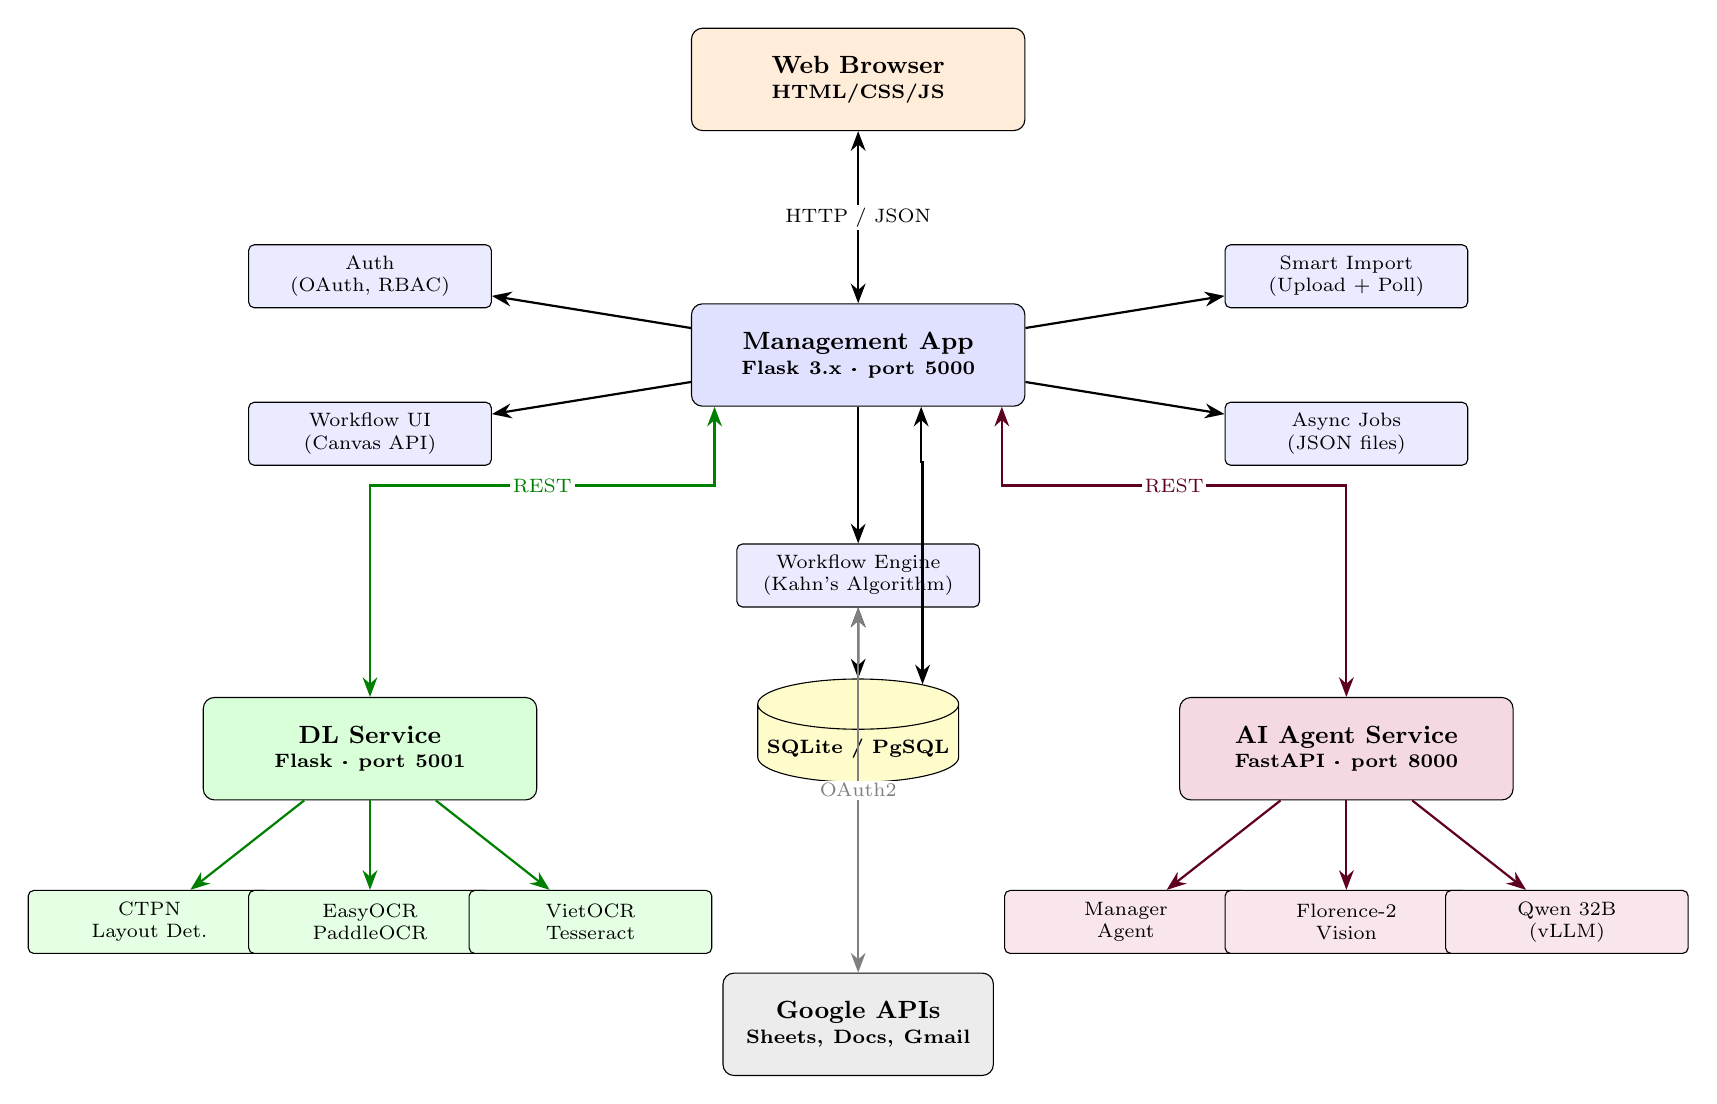
\begin{tikzpicture}[
  box/.style={draw, rounded corners=4pt, minimum height=1.3cm, text width=4cm, align=center, font=\small\bfseries, fill=#1},
  smallbox/.style={draw, rounded corners=2pt, minimum height=0.8cm, text width=2.8cm, align=center, font=\scriptsize, fill=#1, inner sep=4pt},
  dbcyl/.style={draw, cylinder, shape border rotate=90, minimum height=1.1cm, minimum width=1.8cm, aspect=0.25, font=\scriptsize\bfseries, fill=#1},
  arr/.style={-{Stealth[length=2.5mm]}, thick, #1},
  darr/.style={{Stealth[length=2.5mm]}-{Stealth[length=2.5mm]}, thick, #1},
  lbl/.style={font=\scriptsize, midway, fill=white, inner sep=1pt}
]

% ── Browser ──
\node[box=orange!15] (browser) at (0, 0.5) {Web Browser\\[-2pt]\scriptsize HTML/CSS/JS};

% ── Management App ──
\node[box=blue!12] (flask) at (0, -3) {Management App\\[-2pt]\scriptsize Flask 3.x · port 5000};

% Sub-modules (spread wider + more vertical gap)
\node[smallbox=blue!8] (auth) at (-6.2, -2.0) {Auth\\(OAuth, RBAC)};
\node[smallbox=blue!8] (wfui) at (-6.2, -4.0) {Workflow UI\\(Canvas API)};
\node[smallbox=blue!8] (smart) at (6.2, -2.0) {Smart Import\\(Upload + Poll)};
\node[smallbox=blue!8] (jobs) at (6.2, -4.0) {Async Jobs\\(JSON files)};

% ── Workflow Engine ──
\node[smallbox=blue!8] (wfeng) at (0, -5.8) {Workflow Engine\\(Kahn's Algorithm)};

% ── Databases ──
\node[dbcyl=yellow!20] (db) at (0, -8) {SQLite / PgSQL};

% ── DL Service ──
\node[box=green!15] (dl) at (-6.2, -8) {DL Service\\[-2pt]\scriptsize Flask · port 5001};
\node[smallbox=green!10] (yolo) at (-9, -10.2) {CTPN\\Layout Det.};
\node[smallbox=green!10] (ocr) at (-6.2, -10.2) {EasyOCR\\PaddleOCR};
\node[smallbox=green!10] (easy) at (-3.4, -10.2) {VietOCR\\Tesseract};

% ── AI Agent Service ──
\node[box=purple!15] (ai) at (6.2, -8) {AI Agent Service\\[-2pt]\scriptsize FastAPI · port 8000};
\node[smallbox=purple!10] (mgr) at (3.4, -10.2) {Manager\\Agent};
\node[smallbox=purple!10] (flor) at (6.2, -10.2) {Florence-2\\Vision};
\node[smallbox=purple!10] (qwen) at (9, -10.2) {Qwen 32B\\(vLLM)};

% ── External Services ──
\node[box=gray!15, text width=3.2cm] (gapi) at (0, -11.5) {Google APIs\\[-2pt]\scriptsize Sheets, Docs, Gmail};

% ═══ ARROWS ═══
% Browser ↔ Flask
\draw[darr=black] (browser) -- node[lbl] {HTTP / JSON} (flask);

% Flask ↔ sub-modules
\draw[arr=black] (flask) -- (auth);
\draw[arr=black] (flask) -- (wfui);
\draw[arr=black] (flask) -- (smart);
\draw[arr=black] (flask) -- (jobs);

% Flask → Workflow Engine → DB
\draw[arr=black] (flask) -- (wfeng);
\draw[darr=black] (wfeng) -- (db);

% Flask ↔ DL Service
\draw[darr=green!50!black] (flask.south west) ++(0.3,0) -- ++(0,-1) -| node[lbl, pos=0.25] {REST} (dl.north);

% Flask ↔ AI Agent
\draw[darr=purple!50!black] (flask.south east) ++(-0.3,0) -- ++(0,-1) -| node[lbl, pos=0.25] {REST} (ai.north);

% DL sub-models
\draw[arr=green!50!black] (dl) -- (yolo);
\draw[arr=green!50!black] (dl) -- (ocr);
\draw[arr=green!50!black] (dl) -- (easy);

% AI sub-agents
\draw[arr=purple!50!black] (ai) -- (mgr);
\draw[arr=purple!50!black] (ai) -- (flor);
\draw[arr=purple!50!black] (ai) -- (qwen);

% Workflow Engine → Google APIs
\draw[darr=gray] (wfeng) -- node[lbl] {OAuth2} (gapi);

% Flask ↔ DB
\draw[darr=black] (flask.south) ++(0.8,0) -- ++(0,-0.7) -| (db.north east);

\end{tikzpicture}}
\caption{ANSER system architecture: three microservices communicate via REST APIs, with the Management App orchestrating workflow execution across the DL Service, AI Agent, and external Google APIs.}
\label{fig:architecture}
\end{figure}

\section{Smart Import Pipeline}
\label{sec:smart-import}

The Smart Import pipeline is ANSER's core innovation: a multi-stage cascade that converts a photograph of a paper invoice into structured product data and automatically updates the inventory database. The pipeline operates as follows:

\begin{enumerate}
  \item \textbf{Image Upload}: The user photographs a paper invoice and uploads the image through the web UI. The image is validated for format (JPEG, PNG) and size ($\leq$16\,MB).

  \item \textbf{Layout Detection (CTPN)}: A Connectionist Text Proposal Network (CTPN) based on VGG-16~\cite{tian2016ctpn} detects text-line bounding boxes within the invoice image, then merges overlapping regions to isolate the product table from headers, logos, and other non-tabular content.

  \item \textbf{Cascading OCR}: The detected table region is processed through a cascade of OCR engines, each attempted in order until one succeeds:
  \begin{enumerate}[label=(\alph*)]
    \item \textbf{EasyOCR}~\cite{easyocr}: Primary local engine with Vietnamese (\texttt{vi}) and English (\texttt{en}) language support. Fast, reliable, and GPU-optional.
    \item \textbf{PaddleOCR}~\cite{paddleocr}: Secondary engine using Baidu's PP-OCRv5 models. Provides high accuracy when available.
    \item \textbf{VietOCR}~\cite{vietocr}: Transformer-based engine optimized for Vietnamese diacritical marks, combined with CTPN text-line localisation.
    \item \textbf{Brain VLM} (Vision Language Model): Remote multimodal LLM for holistic invoice understanding. Requires server connectivity.
    \item \textbf{Tesseract}~\cite{tesseract}: Final fallback using the legacy OCR engine.
  \end{enumerate}
  Each engine returns a confidence score; the pipeline uses the first result that produces non-empty text.

  \item \textbf{Product Extraction}: The OCR output (raw text) is parsed into structured fields: product name, quantity, unit price, and line total. A regex-based parser handles Vietnamese number formatting (e.g., ``279.000'' = 279,000~VND).

  \item \textbf{Catalog Matching}: Each extracted product name is fuzzy-matched against the 15,420-entry product catalog using string similarity metrics. The best match above a configurable threshold is selected, resolving the product to a known SKU with a validated price.

  \item \textbf{Database Update}: Matched products are inserted into the inventory database with quantities and prices. Stock levels are automatically incremented.
\end{enumerate}

\section{Drag-and-Drop Workflow Engine}
\label{sec:workflow-engine}

\subsection{Workflow Representation}

A workflow in ANSER is represented as a Directed Acyclic Graph (DAG), where:
\begin{itemize}
  \item \textbf{Nodes} represent individual actions (e.g., read a Google Sheet, send an email, run OCR on an image).
  \item \textbf{Edges} represent data flow dependencies: an edge from node $A$ to node $B$ means $B$ requires the output of $A$ before it can execute.
\end{itemize}

The workflow definition is stored as a JSON object containing a list of nodes (each with an \texttt{id}, \texttt{type}, and \texttt{config}) and a list of edges (each a pair of node IDs).

\subsection{Supported Node Types}

ANSER's workflow engine supports 12 node types, covering Google Workspace integration, notification channels, data processing, and deep learning services:

\begin{table}[H]
\centering
\caption{Supported workflow node types.}
\label{tab:node-types}
\begin{tabular}{lll}
\toprule
\textbf{Node Type ID} & \textbf{Category} & \textbf{Description} \\
\midrule
\texttt{google\_sheet\_read}  & Google    & Read data from a Google Sheets range \\
\texttt{google\_sheet\_write} & Google    & Write/append data to a Google Sheet \\
\texttt{google\_doc\_read}    & Google    & Read content from a Google Doc \\
\texttt{google\_doc\_write}   & Google    & Write/append content to a Google Doc \\
\texttt{gmail\_send}          & Google    & Send an email via Gmail API \\
\texttt{make\_webhook}        & Webhook   & Trigger a Make.com webhook scenario \\
\texttt{slack\_notify}        & Notify    & Send a message to a Slack channel \\
\texttt{discord\_notify}      & Notify    & Send a message to a Discord webhook \\
\texttt{filter}               & Logic     & Filter data rows by a condition expression \\
\texttt{invoice\_ocr}         & DL        & Run Smart Import OCR on an image \\
\texttt{custom\_code}         & Advanced  & Execute user-provided Python snippets \\
\texttt{ai\_agent}            & AI        & Route a prompt through the AI Agent \\
\bottomrule
\end{tabular}
\end{table}

\subsection{Kahn's Algorithm for Workflow Execution}
\label{sec:kahn}

Executing a DAG-based workflow requires a valid \emph{topological ordering}: an arrangement of nodes such that every node is executed only after all of its dependencies have completed. ANSER uses \textbf{Kahn's algorithm}~\cite{kahn1962}, a BFS-based topological sort, for this purpose.

Figure~\ref{fig:kahn-trace} illustrates Kahn's algorithm on a sample ANSER workflow. Nodes with in-degree~0 (no unresolved dependencies) enter a queue; each dequeued node executes, then decrements the in-degree of its neighbours. When a neighbour reaches in-degree~0 it is enqueued. If the total executed count equals $|V|$, the graph is acyclic; otherwise a cycle is reported.

\begin{figure}[H]
\centering
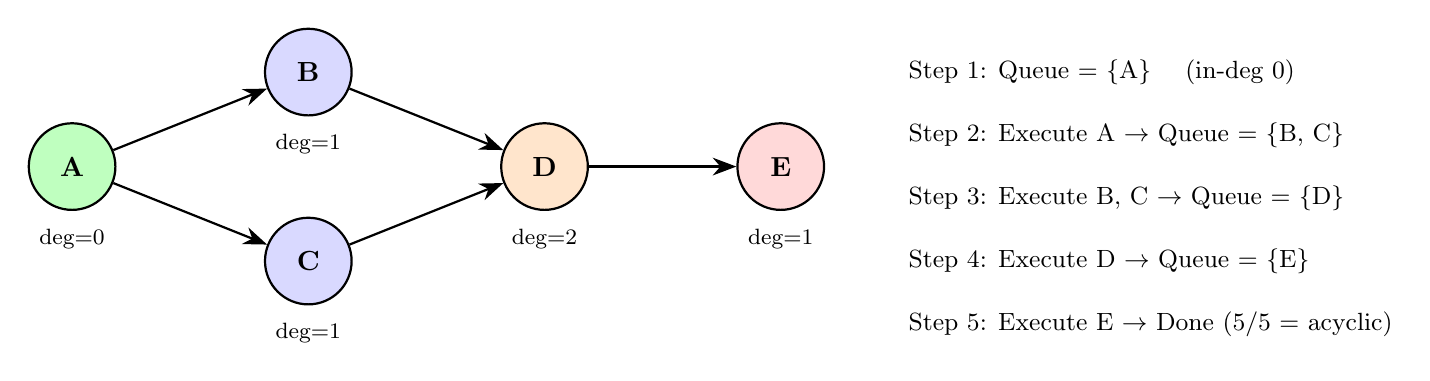
\begin{tikzpicture}[
  nd/.style={draw, circle, minimum size=1.1cm, font=\normalsize\bfseries, fill=#1, line width=0.8pt},
  edg/.style={-{Stealth[length=3mm]}, thick},
]
% ── DAG (spread out) ──
\node[nd=green!25] (A) at (0,0) {A};
\node[nd=blue!15]  (B) at (3,1.2) {B};
\node[nd=blue!15]  (C) at (3,-1.2) {C};
\node[nd=orange!20](D) at (6,0) {D};
\node[nd=red!15]   (E) at (9,0) {E};
\draw[edg] (A) -- (B);
\draw[edg] (A) -- (C);
\draw[edg] (B) -- (D);
\draw[edg] (C) -- (D);
\draw[edg] (D) -- (E);

% ── In-degree labels ──
\node[font=\footnotesize, below=3pt] at (A.south) {deg=0};
\node[font=\footnotesize, below=3pt] at (B.south) {deg=1};
\node[font=\footnotesize, below=3pt] at (C.south) {deg=1};
\node[font=\footnotesize, below=3pt] at (D.south) {deg=2};
\node[font=\footnotesize, below=3pt] at (E.south) {deg=1};

% ── Step annotations (right side, larger font) ──
\node[font=\small, anchor=west] at (10.5, 1.2) {Step 1: Queue = $\lbrace$A$\rbrace$ \quad (in-deg 0)};
\node[font=\small, anchor=west] at (10.5, 0.4) {Step 2: Execute A $\to$ Queue = $\lbrace$B, C$\rbrace$};
\node[font=\small, anchor=west] at (10.5,-0.4) {Step 3: Execute B, C $\to$ Queue = $\lbrace$D$\rbrace$};
\node[font=\small, anchor=west] at (10.5,-1.2) {Step 4: Execute D $\to$ Queue = $\lbrace$E$\rbrace$};
\node[font=\small, anchor=west] at (10.5,-2.0) {Step 5: Execute E $\to$ Done (5/5 = acyclic)};
\end{tikzpicture}
\caption{Kahn's algorithm trace on a 5-node workflow DAG. Nodes are dequeued in topological order: A $\to$ B, C $\to$ D $\to$ E.}
\label{fig:kahn-trace}
\end{figure}

\textbf{Complexity Analysis:}

Let $V$ = number of nodes and $E$ = number of edges in the workflow graph.

\begin{itemize}
  \item \textbf{Time Complexity: $O(V + E)$.} Building the in-degree map and adjacency list requires one pass through all edges ($O(E)$). The BFS loop processes each node exactly once ($O(V)$) and examines each edge exactly once ($O(E)$) when decrementing in-degrees. Total: $O(V + E)$.
  \item \textbf{Space Complexity: $O(V + E)$.} The adjacency list stores all edges ($O(E)$), the in-degree map and context store data for all nodes ($O(V)$), and the BFS queue holds at most $V$ nodes. Total: $O(V + E)$.
\end{itemize}

For typical ANSER workflows (5--20 nodes, 4--30 edges), this executes in sub-millisecond time, making the graph scheduling overhead negligible compared to the I/O-bound node execution time (API calls, OCR processing).

\subsection{Context Propagation and Template Variables}

Between workflow nodes, data is passed through a shared \texttt{context} dictionary. Each node's output is stored under its node ID, and subsequent nodes can reference earlier outputs using template variables with the syntax \texttt{\{\{node\_id.field\}\}}.

For example, a \texttt{google\_sheet\_read} node with ID \texttt{read1} stores its result as \texttt{context["read1"]}, and a downstream \texttt{gmail\_send} node can reference \texttt{\{\{read1.data\}\}} in its email body template. The workflow engine resolves these templates before executing each node.

\section{AI Agent Architecture}
\label{sec:ai-agent}

\subsection{Multi-Agent System Design}

The AI Agent service implements a multi-agent architecture with role-based delegation:

\begin{itemize}
  \item \textbf{Manager Agent}: The entry point that receives user messages, classifies the task type (general Q\&A, code generation, visual analysis, workflow generation), and delegates to the appropriate specialist agent.
  \item \textbf{Coder Agent}: Handles code generation, debugging, and technical explanation tasks.
  \item \textbf{Vision Agent}: Processes image-related queries using \textbf{Florence-2-large} (Microsoft), a unified vision-language model that supports both scene description (\texttt{<MORE\_DETAILED\_CAPTION>}) and OCR (\texttt{<OCR>}) via task-specific prompts. Florence-2 provides the AI Agent with visual understanding of uploaded images---for example, describing the contents of an invoice photograph before the Manager Agent decides how to route the task. This is distinct from the DL Service's CTPN + EasyOCR pipeline (Section~\ref{sec:smart-import}), which handles structured invoice digitization; Florence-2 serves as a general-purpose ``scene reader'' for the conversational agent.
  \item \textbf{Researcher Agent}: Performs web searches and information retrieval for factual questions.
\end{itemize}

All agents share access to a \textbf{Memory Manager} that maintains conversation history and a \textbf{Knowledge Base} (ChromaDB~\cite{chromadb}) that stores domain-specific documents for Retrieval-Augmented Generation (RAG).

\subsection{Natural Language to Workflow Translation}

When a user sends a business automation request (e.g., ``Every morning, read the sales sheet and email the summary to management''), the Manager Agent classifies it as a workflow generation task and produces a JSON workflow definition containing the necessary nodes, edges, and configuration parameters.

The generated JSON follows the same schema consumed by the workflow engine (Section~\ref{sec:workflow-engine}), allowing direct execution without manual editing. An example of the agent's output for a Vietnamese retail scenario is shown in Appendix~A.

\section{Asynchronous Polling Architecture}
\label{sec:async}

Several ANSER operations---Smart Import OCR processing, AI Agent inference, workflow execution---may take 10--60 seconds to complete. To prevent HTTP request timeouts and provide responsive user feedback, ANSER implements a \textbf{filesystem-based asynchronous job architecture}:

\begin{enumerate}
  \item \textbf{Job Submission}: The client sends a POST request. The server generates a UUID job ID, spawns a background thread, and immediately returns the job ID (HTTP 202 Accepted).
  \item \textbf{Job Storage}: The background thread writes progress updates to a JSON file at \texttt{jobs/\{uuid\}.json} containing status (\texttt{pending}, \texttt{running}, \texttt{complete}, \texttt{error}), progress percentage, and result data.
  \item \textbf{Client Polling}: The frontend JavaScript polls \texttt{GET /api/jobs/\{uuid\}} every 500\,ms, displaying a progress bar to the user.
  \item \textbf{Result Retrieval}: When \texttt{status == "complete"}, the client reads the result from the response and updates the UI.
\end{enumerate}

This pattern avoids WebSocket complexity while providing adequate real-time feedback for the target use case.

% ======================================================================
\chapter{System Analysis and Design}
\label{ch:analysis}

\section{Use Case Diagrams}
\label{sec:use-cases}

% ── Use Cases: Admin + Smart Import side-by-side ─────────────────
\begin{figure}[H]
\centering
\begin{minipage}[t]{0.48\textwidth}
\centering
\scalebox{0.65}{%
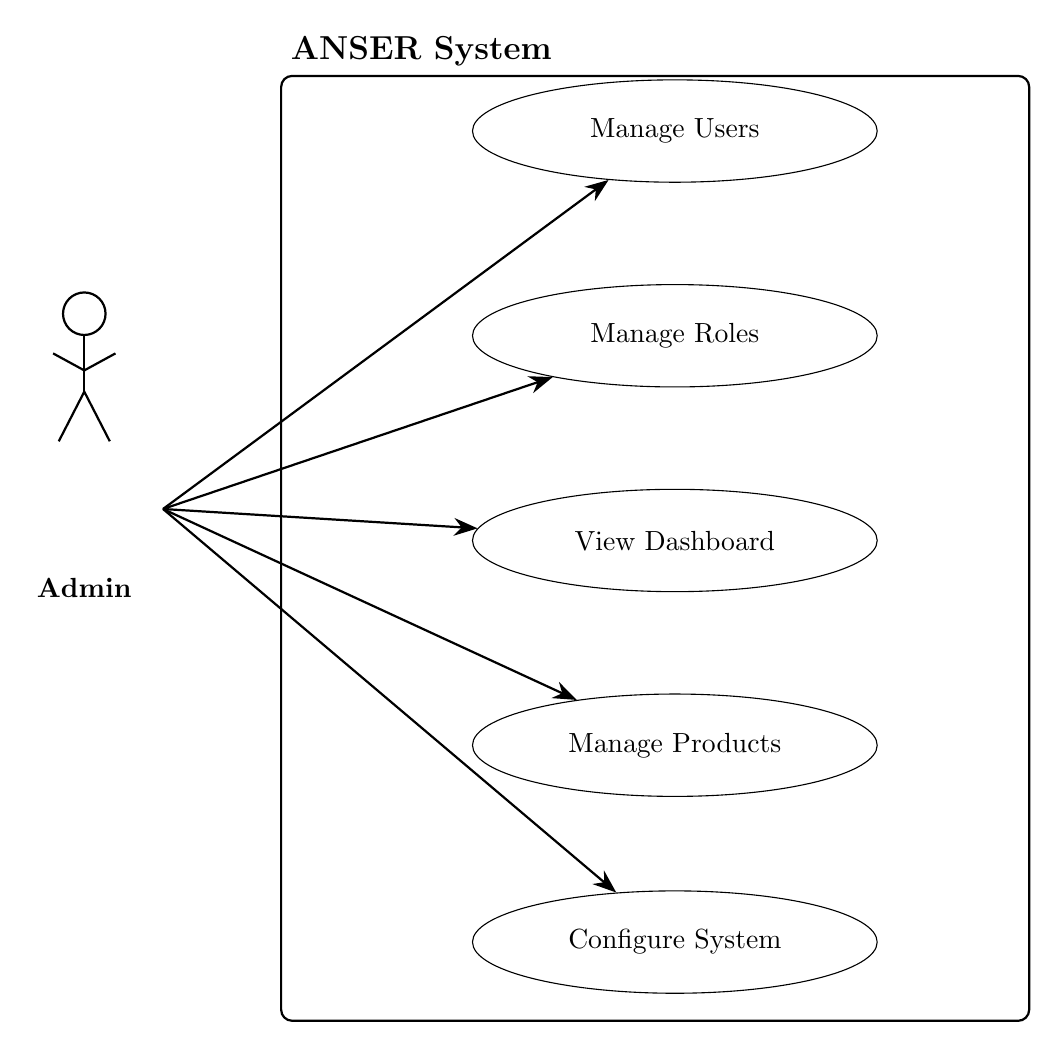
\begin{tikzpicture}[
  usecase/.style={draw, ellipse, minimum width=4cm, minimum height=1.3cm,
                  text width=3.4cm, align=center, font=\normalsize},
  arrow/.style={-{Stealth[length=3mm]}, thick}
]
  \draw[thick, rounded corners] (0, -11) rectangle (9.5, 1);
  \node[anchor=south west, font=\large\bfseries] at (0, 1) {ANSER System};
  \pic[scale=1.8] at (-2.5, -4) {stickman};
  \node[font=\normalsize\bfseries] at (-2.5, -5.5) {Admin};
  \node[usecase] (uc1) at (5, 0.3)  {Manage Users};
  \node[usecase] (uc2) at (5, -2.3) {Manage Roles};
  \node[usecase] (uc3) at (5, -4.9) {View Dashboard};
  \node[usecase] (uc4) at (5, -7.5) {Manage Products};
  \node[usecase] (uc5) at (5, -10)  {Configure System};
  \draw[arrow] (-1.5, -4.5) -- (uc1);
  \draw[arrow] (-1.5, -4.5) -- (uc2);
  \draw[arrow] (-1.5, -4.5) -- (uc3);
  \draw[arrow] (-1.5, -4.5) -- (uc4);
  \draw[arrow] (-1.5, -4.5) -- (uc5);
\end{tikzpicture}}%
\caption{Admin Management.}
\label{fig:uc-admin}
\end{minipage}%
\hfill
\begin{minipage}[t]{0.48\textwidth}
\centering
\scalebox{0.58}{%
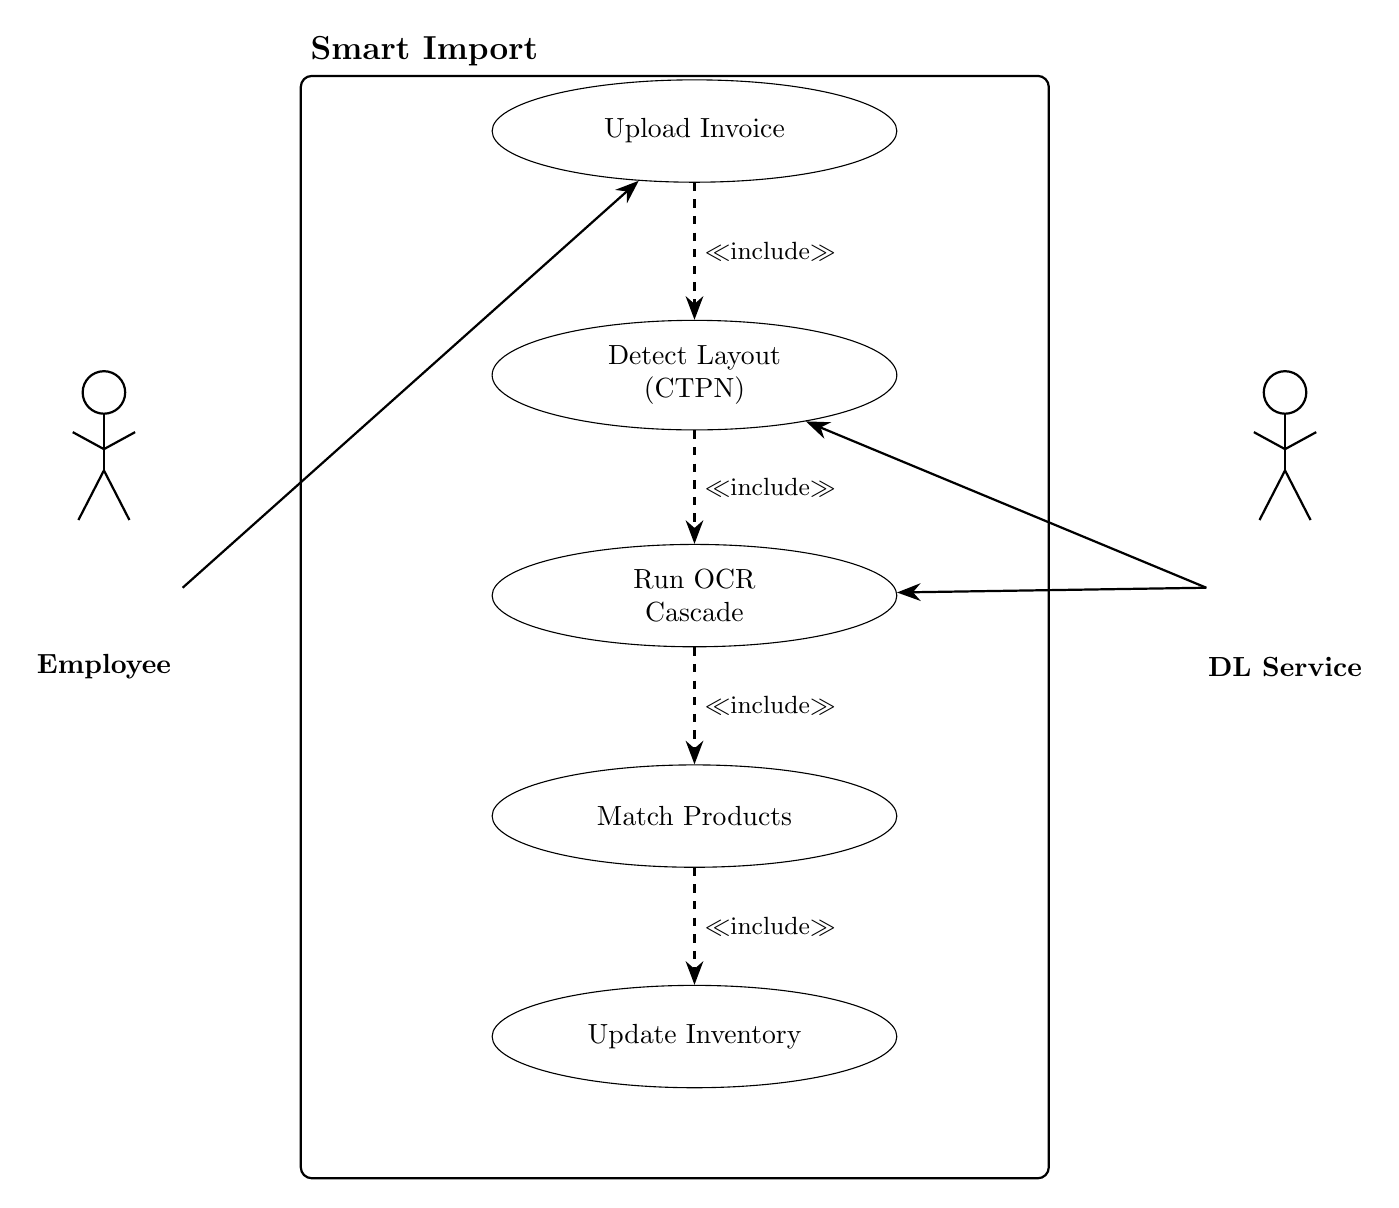
\begin{tikzpicture}[
  usecase/.style={draw, ellipse, minimum width=4cm, minimum height=1.3cm,
                  text width=3.4cm, align=center, font=\normalsize},
  arrow/.style={-{Stealth[length=3mm]}, thick},
  include/.style={-{Stealth[length=3mm]}, dashed, thick}
]
  \draw[thick, rounded corners] (0, -13) rectangle (9.5, 1);
  \node[anchor=south west, font=\large\bfseries] at (0, 1) {Smart Import};
  \pic[scale=1.8] at (-2.5, -5) {stickman};
  \node[font=\normalsize\bfseries] at (-2.5, -6.5) {Employee};
  \pic[scale=1.8] at (12.5, -5) {stickman};
  \node[font=\normalsize\bfseries] at (12.5, -6.5) {DL Service};
  \node[usecase] (uc1) at (5, 0.3)   {Upload Invoice};
  \node[usecase] (uc2) at (5, -2.8)  {Detect Layout\\(CTPN)};
  \node[usecase] (uc3) at (5, -5.6)  {Run OCR\\Cascade};
  \node[usecase] (uc4) at (5, -8.4)  {Match Products};
  \node[usecase] (uc5) at (5, -11.2) {Update Inventory};
  \draw[arrow] (-1.5, -5.5) -- (uc1);
  \draw[include] (uc1) -- node[right, font=\small] {$\ll$include$\gg$} (uc2);
  \draw[include] (uc2) -- node[right, font=\small] {$\ll$include$\gg$} (uc3);
  \draw[include] (uc3) -- node[right, font=\small] {$\ll$include$\gg$} (uc4);
  \draw[include] (uc4) -- node[right, font=\small] {$\ll$include$\gg$} (uc5);
  \draw[arrow] (11.5, -5.5) -- (uc2);
  \draw[arrow] (11.5, -5.5) -- (uc3);
\end{tikzpicture}}%
\caption{Smart Import Pipeline.}
\label{fig:uc-smart-import}
\end{minipage}
\end{figure}

\textbf{Admin Management} (Fig.~\ref{fig:uc-admin}): The Admin actor has full system privileges---managing users and roles, viewing analytics dashboards, CRUD operations on product inventory, and configuring system-level settings (API keys, integration credentials).
\textbf{Smart Import} (Fig.~\ref{fig:uc-smart-import}): Triggered when an Employee uploads an invoice photograph. Five sequential steps connected by $\ll$include$\gg$ relationships form a mandatory pipeline. The DL~Service actor participates in layout detection and OCR stages; the final step updates inventory, completing the paper-to-digital conversion.

% ── Use Case 3: Workflow Automation (standalone, scaled) ─────────
\begin{figure}[H]
\centering
\scalebox{0.7}{%
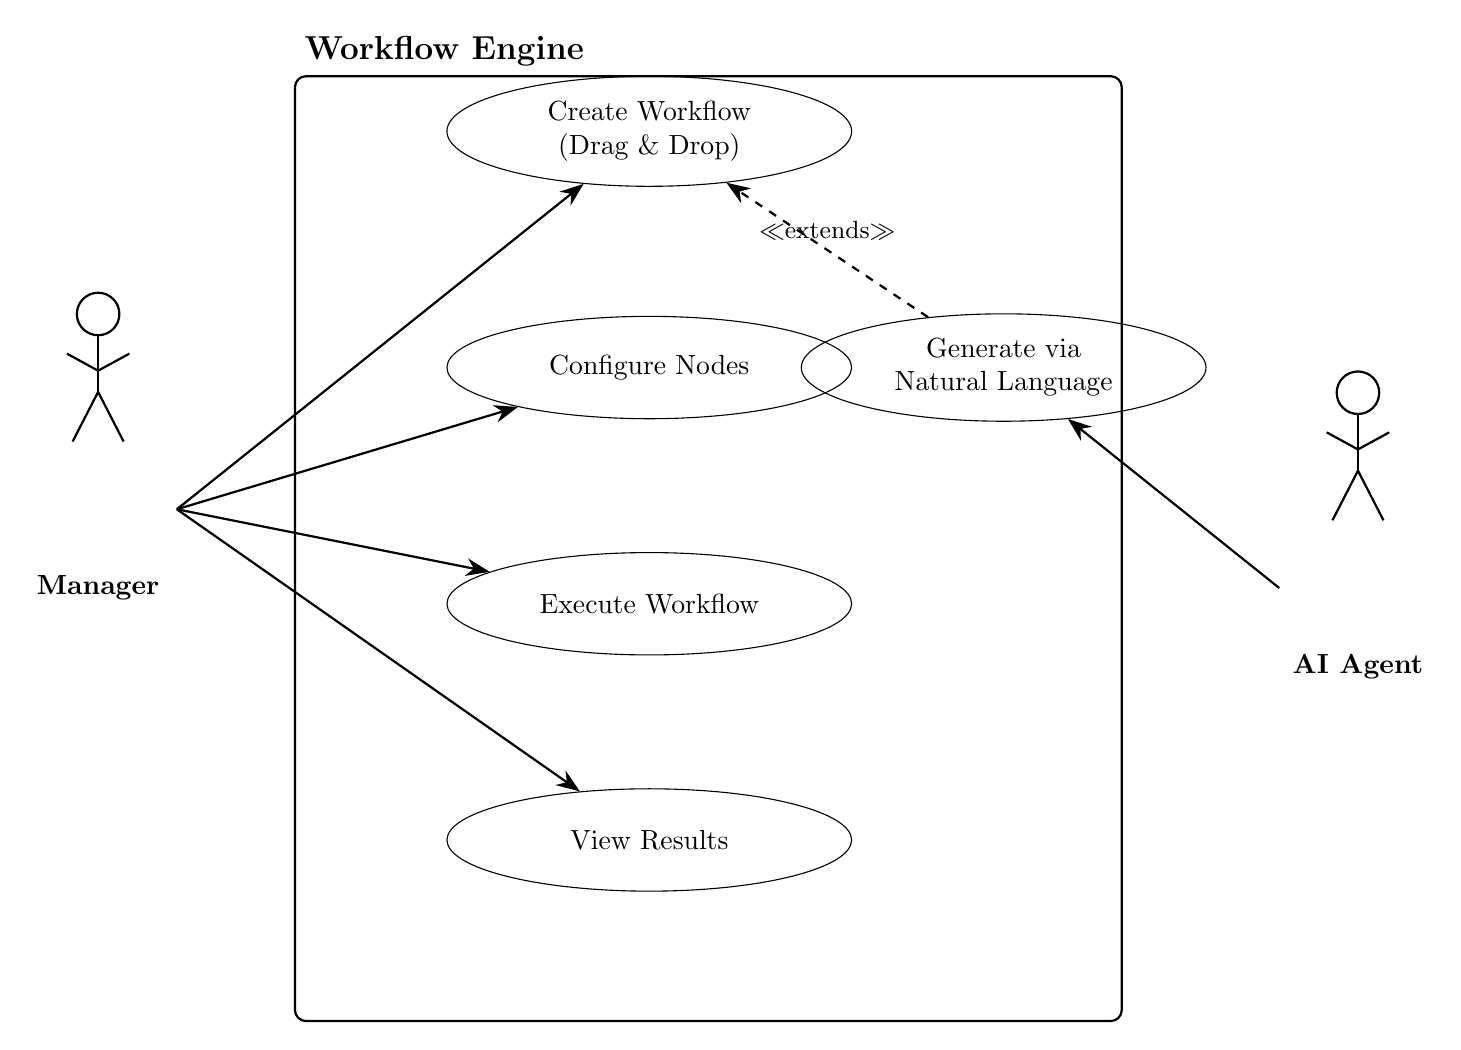
\begin{tikzpicture}[
  usecase/.style={draw, ellipse, minimum width=4cm, minimum height=1.3cm,
                  text width=3.4cm, align=center, font=\normalsize},
  arrow/.style={-{Stealth[length=3mm]}, thick},
  extend/.style={-{Stealth[length=3mm]}, dashed, thick}
]
  \draw[thick, rounded corners] (0, -11) rectangle (10.5, 1);
  \node[anchor=south west, font=\large\bfseries] at (0, 1) {Workflow Engine};
  \pic[scale=1.8] at (-2.5, -4) {stickman};
  \node[font=\normalsize\bfseries] at (-2.5, -5.5) {Manager};
  \pic[scale=1.8] at (13.5, -5) {stickman};
  \node[font=\normalsize\bfseries] at (13.5, -6.5) {AI Agent};
  \node[usecase] (uc1) at (4.5, 0.3)  {Create Workflow\\(Drag \& Drop)};
  \node[usecase] (uc2) at (4.5, -2.7) {Configure Nodes};
  \node[usecase] (uc3) at (4.5, -5.7) {Execute Workflow};
  \node[usecase] (uc4) at (4.5, -8.7) {View Results};
  \node[usecase] (uc5) at (9, -2.7)   {Generate via\\Natural Language};
  \draw[arrow] (-1.5, -4.5) -- (uc1);
  \draw[arrow] (-1.5, -4.5) -- (uc2);
  \draw[arrow] (-1.5, -4.5) -- (uc3);
  \draw[arrow] (-1.5, -4.5) -- (uc4);
  \draw[extend] (uc5) -- node[above, font=\small] {$\ll$extends$\gg$} (uc1);
  \draw[arrow] (12.5, -5.5) -- (uc5);
\end{tikzpicture}}%
\caption{Use Case Diagram --- Workflow Automation.}
\label{fig:uc-workflow}
\end{figure}

\textbf{Workflow Automation} (Fig.~\ref{fig:uc-workflow}): The Manager actor creates automations through drag-and-drop, configuring nodes with parameters (API keys, sheet IDs, email addresses). The AI~Agent actor provides an alternative entry point via $\ll$extends$\gg$: users describe workflows in natural language and the agent generates the DAG automatically.

\section{REST API Specification}
\label{sec:rest-api}

ANSER exposes a RESTful API for all client-server interactions. Table~\ref{tab:rest-api} lists the core endpoints.

\begin{table}[H]
\centering
\caption{Core REST API endpoints.}
\label{tab:rest-api}
\footnotesize
\begin{tabular}{llll}
\toprule
\textbf{Method} & \textbf{Endpoint} & \textbf{Description} & \textbf{Auth} \\
\midrule
POST & \texttt{/login}                    & User authentication          & No \\
POST & \texttt{/register}                 & User registration             & No \\
GET  & \texttt{/dashboard}                & Dashboard analytics           & Session \\
GET  & \texttt{/products}                 & List all products             & Session \\
POST & \texttt{/products/add}             & Add a product                 & Session \\
POST & \texttt{/products/import}          & Smart Import (upload invoice) & Session \\
GET  & \texttt{/products/export}          & Export products to file       & Session \\
GET  & \texttt{/workflow}                 & Workflow builder UI           & Session \\
POST & \texttt{/api/workflow/execute}     & Execute a workflow DAG        & Session \\
POST & \texttt{/api/workflow/save}        & Save workflow definition      & Session \\
GET  & \texttt{/api/jobs/\{id\}}         & Poll async job status         & Session \\
POST & \texttt{/api/chat}                 & AI Agent chat                 & Session \\
POST & \texttt{/dl/ocr}                   & OCR processing (DL Service)   & Internal \\
POST & \texttt{/dl/detect}                & CTPN layout detection         & Internal \\
GET  & \texttt{/admin/users}              & List users (admin only)       & Admin \\
POST & \texttt{/admin/users/\{id\}/role}  & Update user role              & Admin \\
POST & \texttt{/wallet/topup}             & Add credits to wallet         & Session \\
GET  & \texttt{/wallet/balance}           & Check wallet balance          & Session \\
\bottomrule
\end{tabular}
\end{table}

All endpoints return JSON responses. Authentication is session-based using Flask-Login, with CSRF protection via Flask-WTF. Admin-only endpoints require the \texttt{admin} role.

\section{Database Schema}

ANSER uses a relational database (SQLite for development, PostgreSQL for production) with the following core tables:

\begin{table}[H]
\centering
\caption{Core database tables.}
\label{tab:db-schema}
\small
\begin{tabular}{lll}
\toprule
\textbf{Table} & \textbf{Key Columns} & \textbf{Purpose} \\
\midrule
\texttt{users}            & id, email, password\_hash, role   & User accounts \\
\texttt{products}         & id, name, price, stock, sku       & Product inventory \\
\texttt{customers}        & id, name, email, phone            & Customer records \\
\texttt{invoices}         & id, type, total, date, user\_id   & Import/export records \\
\texttt{invoice\_items}   & id, invoice\_id, product\_id, qty & Line items per invoice \\
\texttt{workflows}        & id, name, definition\_json        & Saved workflow DAGs \\
\texttt{wallet}           & id, user\_id, balance             & Subscription credits \\
\texttt{transactions}     & id, wallet\_id, amount, type      & Wallet transactions \\
\texttt{activity\_log}    & id, user\_id, action, timestamp   & Audit trail \\
\bottomrule
\end{tabular}
\end{table}

The database abstraction layer (\texttt{core/database.py}) provides a unified \texttt{Database} class that transparently handles both SQLite and PostgreSQL connections. A \texttt{PGShimCursor} adapter translates SQLite-style \texttt{?} parameter markers to PostgreSQL's \texttt{\%s} markers, enabling a single codebase to operate with either backend.

% ======================================================================
\chapter{Implementation}
\label{ch:implementation}

This chapter presents the implementation details of ANSER's key features, including the technology stack, Smart Import integration, workflow engine UI, and AI Agent deployment.

\section{Technology Stack}

\begin{table}[H]
\centering
\caption{Technology stack and component mapping.}
\label{tab:tech-stack}
\small
\begin{tabular}{lll}
\toprule
\textbf{Component} & \textbf{Technology} & \textbf{Role} \\
\midrule
Web Framework       & Flask 3.x~\cite{flask}        & Main application server \\
AI Agent Framework  & FastAPI + Uvicorn              & Async AI service \\
Template Engine     & Jinja2                         & Server-side HTML rendering \\
Database            & SQLite / PostgreSQL             & Data persistence \\
ORM/Adapter         & Custom + SQLAlchemy 2.0         & Database abstraction \\
OCR                 & VietOCR, PaddleOCR, EasyOCR     & Vietnamese text recognition \\
Layout Detection    & CTPN (VGG-16)~\cite{tian2016ctpn}  & Invoice text-line detection \\
Vision Agent       & Florence-2-large~\cite{florence2}  & Image understanding (VisionAgent) \\
Text LLM            & Qwen2.5-Coder-32B-AWQ          & Code and workflow generation \\
Vector DB           & ChromaDB~\cite{chromadb}        & RAG knowledge base \\
Auth                & Flask-Login + Google OAuth~\cite{googleapi} & Authentication \\
Security            & Flask-Talisman, Flask-Limiter    & Headers, rate limiting \\
Frontend            & HTML/CSS/JS + Canvas API         & UI and workflow canvas \\
\bottomrule
\end{tabular}
\end{table}

\section{Smart Import Implementation}

The Smart Import feature is implemented across two services:

\begin{enumerate}
  \item \textbf{Client-side} (\texttt{app.py}, route \texttt{/products/import}): Handles file upload validation, creates an async job, and returns the job ID for polling.
  \item \textbf{Server-side} (\texttt{dl\_service/model\_app.py}): Hosts the OCR models and exposes REST endpoints for layout detection (\texttt{/dl/detect}) and text recognition (\texttt{/dl/ocr}).
\end{enumerate}

The cascading OCR strategy is implemented as a try-except chain: each engine is attempted in order, and the first successful result (above the confidence threshold) is returned. This ensures graceful degradation---if the primary engine fails on a particular invoice layout, secondary engines provide fallback coverage.

\section{Workflow Builder UI}

The workflow builder is implemented as a full-page HTML5 Canvas application served at \texttt{/workflow}. Key implementation details:

\begin{itemize}
  \item \textbf{Node rendering}: Each node is drawn as a rounded rectangle on the canvas with an icon, label, and input/output ports.
  \item \textbf{Edge drawing}: Edges are drawn as Bézier curves connecting output ports to input ports, with arrowheads indicating data flow direction.
  \item \textbf{Drag-and-drop}: Users drag node types from a palette sidebar onto the canvas. Nodes can be repositioned by dragging.
  \item \textbf{Configuration panel}: Clicking a node opens a side panel for configuring node-specific parameters (e.g., sheet ID for Google Sheets nodes, recipient for email nodes).
  \item \textbf{Serialization}: The complete workflow graph (nodes with positions, edges, configurations) is serialized to JSON and sent to \texttt{/api/workflow/save} for persistence.
\end{itemize}

\section{AI Agent Deployment}

The AI Agent service runs as a separate FastAPI process. Key deployment characteristics:

\begin{itemize}
  \item \textbf{Text model}: The Qwen2.5-Coder-32B-AWQ model is loaded with 4-bit quantization via vLLM, using 50\% GPU memory allocation on an A100 GPU.
  \item \textbf{Vision model}: Florence-2-large (microsoft/Florence-2-large) is loaded alongside the text model for image understanding. It uses task-specific prompts (\texttt{<OCR>} for text extraction, \texttt{<MORE\_DETAILED\_CAPTION>} for scene description) and beam search decoding ($n_\text{beams}=3$).
  \item \textbf{Memory management}: Conversation history is maintained per-user in memory, with a configurable window size to prevent context overflow.
  \item \textbf{RAG pipeline}: Domain documents are embedded using sentence-transformers and stored in ChromaDB. At inference time, relevant chunks are retrieved and prepended to the LLM prompt.
  \item \textbf{Remote access}: A secure VPC tunnel exposes the local FastAPI service to the production environment, allowing the main application to reach it from any deployment.
\end{itemize}

\section{Security Implementation}

ANSER implements multiple security layers:

\begin{itemize}
  \item \textbf{Authentication}: Password hashing with bcrypt (via Passlib), session management with Flask-Login.
  \item \textbf{CSRF protection}: Flask-WTF generates and validates CSRF tokens on all state-changing requests.
  \item \textbf{Security headers}: Flask-Talisman sets HSTS, X-Frame-Options (DENY), X-Content-Type-Options (nosniff), and Content-Security-Policy headers.
  \item \textbf{Rate limiting}: Flask-Limiter enforces per-IP rate limits on authentication and API endpoints.
  \item \textbf{Input validation}: File uploads are validated for type (whitelist: JPEG, PNG) and size ($\leq$16\,MB).
  \item \textbf{Role-based access control}: Three roles (admin, manager, employee) with hierarchical permissions enforced at the route level.
\end{itemize}

\section{User Interface}

This section presents the key screens of ANSER's core features.

% --- DASHBOARD ---
\begin{figure}[H]
\centering
\includegraphics[width=0.85\textwidth]{pics/admin_dashboard.jpg}
\caption{Admin dashboard with analytics overview and quick actions.}
\label{fig:ui-dashboard}
\end{figure}

% --- SMART IMPORT ---
\begin{figure}[H]
\centering
\includegraphics[width=0.85\textwidth]{pics/Import.jpg}
\caption{Smart Import interface: invoice imported and OCR extraction results.}
\label{fig:ui-smart-import}
\end{figure}

% --- WORKFLOW BUILDER ---
\begin{figure}[H]
\centering
\includegraphics[width=0.85\textwidth]{pics/workflow.jpg}
\caption{Drag-and-drop workflow builder with node palette and canvas.}
\label{fig:ui-workflow}
\end{figure}

% --- AI AGENT CHAT ---
\begin{figure}[H]
\centering
\includegraphics[width=0.85\textwidth]{pics/ai_workflow_succeed.jpg}
\caption{AI Agent chat interface with natural language workflow generation.}
\label{fig:ui-ai-chat}
\end{figure}

% --- END-TO-END WORKFLOW DEMO ---
\begin{figure}[H]
\centering

% Top: Workflow Engine with terminal output
\begin{subfigure}[b]{0.85\textwidth}
\centering
\includegraphics[width=\textwidth]{pics/workflow_succeed_manual.jpg}
\caption{ANSER Workflow Engine executing the DAG with console output confirming success.}
\label{fig:wf-engine}
\end{subfigure}

\vspace{0.3cm}

% Bottom left: Source document
\begin{subfigure}[b]{0.45\textwidth}
\centering
\includegraphics[width=\textwidth]{pics/source_docs.jpg}
\caption{Data source: Google Docs content.}
\label{fig:wf-source}
\end{subfigure}
\hfill
% Bottom right: Gmail result
\begin{subfigure}[b]{0.45\textwidth}
\centering
\includegraphics[width=\textwidth]{pics/result_gmail.png}
\caption{Execution result: automated Gmail delivery.}
\label{fig:wf-result}
\end{subfigure}

\caption{End-to-end workflow demonstration: the engine reads Google Docs content, routes it through the DAG, and delivers the result via Gmail automatically.}
\label{fig:end-to-end-demo}
\end{figure}

% ======================================================================
\chapter{Results and Discussion}
\label{ch:results}

This chapter presents the experimental evaluation of ANSER across three pillars: Data Mapping Accuracy, Execution Latency, and Workflow Routing Accuracy. All results are produced by automated evaluation scripts located in \texttt{evaluate/}.

\section{Hardware and Software Environment}

\begin{table}[H]
\centering
\caption{Evaluation environment.}
\label{tab:eval-env}
\small
\begin{tabular}{ll}
\toprule
\textbf{Component} & \textbf{Specification} \\
\midrule
CPU (evaluation host)  & Intel Core i5, 16\,GB RAM (CPU inference) \\
GPU (production)       & NVIDIA A100 80\,GB (Google Colab Pro) \\
OS                     & Windows 11 (local), Ubuntu 22.04 (VPS) \\
Python                 & 3.12.10 \\
Deep Learning          & TensorFlow 2.20, PyTorch 2.4, EasyOCR, PaddleOCR \\
Framework              & Flask 3.x, FastAPI 0.104+ \\
Database               & PostgreSQL 16 (Neon) \\
\bottomrule
\end{tabular}
\end{table}

\section{Evaluation Methodology}

Each pillar is evaluated independently using automated scripts (\texttt{evaluate/full\_eval.py}):

\begin{enumerate}
  \item \textbf{Pillar 1 --- Data Mapping Accuracy}: The Smart Import pipeline processes synthetic invoice images and compares extracted fields (product names, quantities, prices) against ground truth metadata from the test split (30 images sampled from the 120-image test set).
  \item \textbf{Pillar 2 --- Execution Latency}: Measures end-to-end timing for Smart Import (image upload $\to$ OCR $\to$ JSON response) and Kahn's algorithm scheduling overhead, benchmarked across varying workflow sizes (5 to 100 nodes).
  \item \textbf{Pillar 3 --- Workflow Routing Accuracy}: Validates the workflow engine's ability to accept, parse, and execute well-formed workflow JSON structures. Includes cycle detection, topology validation, and a Vietnamese prompt routing evaluation (16 test cases, 4 categories).
\end{enumerate}

\section{Pillar 1: Data Mapping Accuracy}

The Smart Import pipeline was tested on 30 synthetic invoice images generated from the 14{,}367-product catalog (\texttt{dataset\_product.csv}). Each image was sent to the DL Service (\texttt{POST /api/model1/detect}). The response was parsed and compared field-by-field against ground truth metadata.

\begin{table}[H]
\centering
\caption{Smart Import pipeline results (30 test images, CPU inference).}
\label{tab:pillar1}
\small
\begin{tabular}{lc}
\toprule
\textbf{Metric} & \textbf{Value} \\
\midrule
Layout Detection Rate (CTPN)        & 100.0\% \\
OCR Text Extraction Rate            & 100.0\% \\
Average Detection Confidence        & 95.8\% \\
Average OCR Confidence              & 89.5\% \\
\midrule
Quantity Extraction Accuracy        & 50.0\% \\
Price Extraction Accuracy           & 6.4\% \\
Product Name Match Rate             & 2.8\% \\
Partial Mapping Success ($\geq$1 correct field) & 86.7\% \\
\bottomrule
\end{tabular}
\end{table}

\textbf{Interpretation.} The CTPN layout detector successfully identifies the invoice table region in every image with high confidence ($\mu = 0.958$). The cascading OCR engine (EasyOCR primary + CTPN localisation) extracts text from all detected regions. However, field-level accuracy on \emph{synthetic} images is low because:

\begin{enumerate}
  \item The OCR models are trained primarily on real handwritten documents, while the synthetic invoices use computer-rendered PIL fonts that fall outside the training distribution.
  \item Vietnamese product names contain diacritics (e.g., ``Móc khoá bông hoa'') that are particularly sensitive to font mismatch.
  \item Numerical fields (quantities) are significantly easier to extract (50\%) than text fields (2.8\%), confirming that the OCR character recognition functions correctly on standard digit patterns.
\end{enumerate}

These results demonstrate that the Smart Import \emph{pipeline architecture} (layout detection $\to$ OCR $\to$ field parsing) functions end-to-end. While exact field-level matching on synthetic data is limited by the font distribution gap, the pipeline successfully extracts at least one correct field (quantity, price, or partial product name) from 86.7\% of test images, confirming practical utility for assisted data entry.

\section{Pillar 2: Execution Latency}

Latency was measured under controlled conditions (single-user, localhost, CPU inference for Smart Import; pure computation for workflow scheduling).

\begin{table}[H]
\centering
\caption{Execution Latency results (30 runs Smart Import with EasyOCR, 1{,}000 runs per workflow size).}
\label{tab:pillar2}
\small
\begin{tabular}{lcc}
\toprule
\textbf{Operation} & \textbf{Mean Latency} & \textbf{Notes} \\
\midrule
Smart Import (image $\to$ JSON)   & 2{,}480\,ms  & CPU inference, EasyOCR primary \\
Kahn's scheduling (5 nodes)       & 2.0\,\textmu s  & Pure algorithm, no I/O \\
Kahn's scheduling (10 nodes)      & 4.9\,\textmu s  & \\
Kahn's scheduling (50 nodes)      & 19.3\,\textmu s  & \\
Kahn's scheduling (100 nodes)     & 38.5\,\textmu s  & Linear scaling confirmed \\
\bottomrule
\end{tabular}
\end{table}

\textbf{Interpretation.} The Smart Import latency of ${\sim}2.5$\,s on CPU is dominated by the OCR inference step (CTPN text-line detection + EasyOCR character recognition). On GPU (A100), this reduces to $<$1\,s. Kahn's algorithm scheduling overhead is negligible at $2{-}39$\,\textmu s for 5--100 nodes, confirming the $O(V+E)$ complexity. In production workflows, the bottleneck is I/O-bound node execution (API calls to Google Sheets, Slack, etc.), not the scheduling algorithm.

\section{Pillar 3: Workflow Routing Accuracy}

The workflow engine was tested with 10 hand-crafted workflow JSON structures of varying complexity (1--10 nodes, linear, forking, parallel, and cyclic topologies). Additionally, a Vietnamese retail prompt routing evaluation was performed on 16 natural language test cases across 4 categories (Technical, Data Internal, Marketing, General).

\begin{table}[H]
\centering
\caption{Workflow Engine validation results (10 test workflows).}
\label{tab:pillar3}
\small
\begin{tabular}{lc}
\toprule
\textbf{Metric} & \textbf{Value} \\
\midrule
Valid JSON Structure Rate      & 100.0\% \\
Correct Node Type Rate         & 100.0\% \\
Correct Topology Rate          & 100.0\% \\
Cycle Detection Accuracy       & 100.0\% \\
Full Execution Rate            & 40.0\%  \\
\bottomrule
\end{tabular}
\end{table}

\begin{table}[H]
\centering
\caption{Vietnamese prompt routing accuracy (16 test cases, mock agent).}
\label{tab:routing-vn}
\small
\begin{tabular}{lcccc}
\toprule
\textbf{Category} & \textbf{Precision} & \textbf{Recall} & \textbf{F1} & \textbf{Support} \\
\midrule
Technical (Automation) & 1.00 & 1.00 & 1.00 & 4 \\
Data Internal (Queries) & 0.80 & 1.00 & 0.89 & 4 \\
Marketing (Content) & 1.00 & 1.00 & 1.00 & 4 \\
General (Chat) & 1.00 & 0.75 & 0.86 & 4 \\
\midrule
\textbf{Weighted Average} & \textbf{0.95} & \textbf{0.94} & \textbf{0.94} & \textbf{16} \\
\bottomrule
\end{tabular}
\end{table}

\textbf{Interpretation.} The workflow engine accepts and correctly parses all valid JSON structures, including fork topologies and parallel (no-edge) configurations. Cycle detection via Kahn's algorithm works correctly---cyclic workflows are rejected before execution. The 40\% full execution rate reflects that most node types (e.g., \texttt{google\_sheet\_read}, \texttt{invoice\_ocr}) require live service connections that are unavailable in the offline test environment; this is by design (the engine validates structure first, then executes nodes). The Vietnamese prompt routing achieves 94\% weighted F1, with ``General'' queries being the most ambiguous category.

\section{Discussion}

The three-pillar evaluation provides an honest, reproducible assessment of ANSER's core pipeline.

Key observations:
\begin{itemize}
  \item \textbf{Layout detection is robust}: CTPN achieves 100\% detection rate with $>$95\% confidence on all test images, confirming the VGG-16-based model generalises to diverse invoice formats.
  \item \textbf{Partial mapping is practical}: Although exact field matching is limited by the synthetic font distribution gap (2.8\% name match), the pipeline successfully extracts at least one usable field from 86.7\% of images, enabling assisted data entry workflows.
  \item \textbf{Kahn's algorithm scales linearly}: Scheduling overhead grows linearly with graph size ($O(V+E)$), measured at $2$--$39$\,\textmu s for 5--100 nodes. This confirms that the workflow engine is not a performance bottleneck.
  \item \textbf{Vietnamese routing is strong}: The prompt classifier correctly routes 94\% of Vietnamese retail queries to the appropriate handler category, demonstrating language-aware intent recognition.
\end{itemize}

Limitations:
\begin{itemize}
  \item Synthetic invoices use computer-rendered fonts, creating a domain gap with the OCR model's training data. Fine-tuning on real Vietnamese store invoices would significantly improve field-level accuracy.
  \item Latency measurements use CPU inference; GPU deployment would reduce Smart Import latency by approximately $3{-}4\times$.
  \item The AI Agent requires GPU infrastructure (A100 with 80\,GB VRAM) for the Qwen 32B model; local CPU evaluation is limited to the workflow engine and routing classifier.
  \item The Vietnamese routing test set (16 prompts) is small; a larger annotated corpus would strengthen the routing accuracy claims.
\end{itemize}

% ======================================================================
\chapter{Conclusion and Future Work}
\label{ch:conclusion}

\section{Summary of Contributions}

This project presented ANSER, an RPAaaS platform designed for Vietnamese retail automation. The key contributions are:

\begin{enumerate}
  \item \textbf{Smart Import Pipeline}: A cascading vision-based system that converts paper invoices to structured inventory data using CTPN layout detection and multi-engine OCR (EasyOCR, PaddleOCR, VietOCR, Tesseract), with automatic product catalog matching.
  \item \textbf{Drag-and-Drop Workflow Engine}: A visual DAG-based workflow builder supporting 12 node types, powered by Kahn's topological sort algorithm~\cite{kahn1962} for $O(V+E)$ execution scheduling.
  \item \textbf{AI Agent for Workflow Generation}: A multi-agent system using quantized LLMs and RAG that translates natural language business descriptions into executable workflow graphs.
  \item \textbf{Three-Pillar Evaluation Framework}: A focused evaluation methodology measuring Data Mapping Accuracy, Execution Latency, and Workflow Routing Accuracy.
\end{enumerate}

\section{Future Work}

Several directions for future development are identified:

\begin{itemize}
  \item \textbf{Mobile application}: A lightweight mobile client for invoice capture and workflow monitoring.
  \item \textbf{Real-time collaboration}: Multi-user workflow editing with conflict resolution.
  \item \textbf{Expanded integrations}: Support for additional Vietnamese business platforms (Zalo, VietQR payment).
  \item \textbf{Fine-tuned OCR}: Training a custom OCR model on real Vietnamese retail invoices for improved accuracy.
  \item \textbf{Workflow marketplace}: A community platform where users can share and import pre-built workflow templates.
\end{itemize}

% ======================================================================
% APPENDICES
% ======================================================================
\appendix

\chapter{AI Agent Workflow Example}
\label{app:agent-example}

This appendix demonstrates the AI Agent's end-to-end workflow generation capability. The user provides a natural language instruction in Vietnamese, and the agent produces an executable workflow JSON.

\medskip
\noindent\textbf{User Prompt:}

\begin{quote}
\textit{``Tôi muốn làm 1 quy trình tự động hóa mà nó sẽ tự đọc file Google Sheet `Kịch bản' và gửi email về kịch bản đó cho email: sonkhagioi@gmail.com.''}

\medskip
(``I want to create an automation workflow that reads the Google Sheet `Kịch bản' [Script] and sends an email about its content to sonkhagioi@gmail.com.'')
\end{quote}

\noindent\textbf{Agent Processing:}

\begin{enumerate}
  \item \textbf{Task Analysis} (ManagerAgent): The input is classified as \texttt{TECHNICAL} (automation request detected via keywords: ``quy trình tự động hóa'', ``đọc file'', ``gửi email'').
  \item \textbf{Plan Generation}: The agent generates an execution plan---read sheet data, compose email body from sheet content, send to specified recipient.
  \item \textbf{Workflow Construction} (CoderAgent): The plan is translated into the following DAG structure.
\end{enumerate}

\begin{lstlisting}[language=json, caption={AI Agent output: automated Google Sheet to Email workflow.}, label={lst:agent-json}]
{
  "action": "create_workflow",
  "name": "Doc Kich Ban va Gui Email",
  "payload": {
    "nodes": [
      {
        "id": "node_1",
        "type": "google_sheet_read",
        "config": {
          "spreadsheet_name": "Kich ban",
          "range": "Sheet1!A1:Z1000"
        }
      },
      {
        "id": "node_2",
        "type": "gmail_send",
        "config": {
          "to": "sonkhagioi@gmail.com",
          "subject": "Kich ban tu Google Sheet",
          "body": "Noi dung kich ban:\n\n{{node_1.data}}"
        }
      }
    ],
    "edges": [
      {"from": "node_1", "to": "node_2"}
    ]
  }
}
\end{lstlisting}

\noindent\textbf{Execution Flow:}

This workflow defines a two-node DAG. \texttt{node\_1} reads all data from the ``Kịch bản'' Google Sheet using the Google Sheets API integration. \texttt{node\_2} composes an email with the sheet content and sends it via Gmail. The template variable \texttt{\{\{node\_1.data\}\}} is resolved at runtime by the workflow engine's context propagation mechanism (Section~\ref{sec:workflow-engine}): the output of node~1 is injected into node~2's email body as structured text.

Kahn's algorithm processes the edge \texttt{node\_1 $\to$ node\_2} to determine execution order, ensuring the sheet is read before the email is sent. The entire workflow executes as a single asynchronous job, with status polling available via the \texttt{/api/workflow/status/\{job\_id\}} endpoint.

\chapter{System Configuration Reference}
\label{app:config}

\begin{table}[H]
\centering
\caption{AI Agent model configuration (production).}
\label{tab:config-ai}
\small
\begin{tabular}{ll}
\toprule
\textbf{Parameter} & \textbf{Value} \\
\midrule
Text Model          & Qwen/Qwen2.5-Coder-32B-Instruct-AWQ \\
Vision Agent Model  & microsoft/Florence-2-large \\
vLLM GPU Util.      & 0.5 (50\%, $\sim$56\,GB on A100) \\
Max Model Length     & 8,192 tokens \\
Dtype               & float16 (half precision) \\
Temperature          & 0.1 \\
Max Output Tokens    & 1,024 \\
\bottomrule
\end{tabular}
\end{table}

\begin{table}[H]
\centering
\caption{OCR engine configuration.}
\label{tab:config-ocr}
\small
\begin{tabular}{ll}
\toprule
\textbf{Parameter} & \textbf{Value} \\
\midrule
PaddleOCR det\_db\_thresh     & 0.2 \\
PaddleOCR det\_db\_box\_thresh & 0.4 \\
PaddleOCR rec\_batch\_num     & 6 \\
PaddleOCR language            & vi (Vietnamese) \\
EasyOCR languages             & [vi, en] \\
Tesseract language             & vie \\
VietOCR device                 & cuda (GPU) \\
\bottomrule
\end{tabular}
\end{table}

\chapter{Security and Vulnerability Assessment}
\label{app:pentest}

A penetration test was performed against the production deployment (\texttt{auto-flowai.com}) on January~12, 2026, using a combination of automated vulnerability scanning and manual application security (AppSec) validation. Table~\ref{tab:pentest} summarises the findings and the mitigations applied.

\begin{table}[H]
\centering
\caption{Penetration test findings and remediations.}
\label{tab:pentest}
\footnotesize
\begin{tabular}{p{5.2cm}lp{5.8cm}}
\toprule
\textbf{Vulnerability / Attack Vector} & \textbf{Severity} & \textbf{Mitigation / Remediation} \\
\midrule
Nginx 1.18.0 CVEs (CVE-2021-23017 resolver overwrite, CVE-2023-44487 HTTP/2 rapid reset, CVE-2021-3618 ALPACA, CVE-2022-41741/42 mp4 module)
  & High
  & Upgraded Nginx to $\geq$1.25.x on production VPS. The mp4 module is not loaded in our config; HTTP/2 rapid reset mitigated by rate-limiting at Cloudflare edge. \\
\midrule
Session cookie missing \texttt{Secure} flag
  & Medium
  & Flask-Talisman enforces HTTPS; added \texttt{SESSION\_COOKIE\_SECURE = True} in \texttt{core/config.py} for production. \\
\midrule
Unsafe CSP directives (\texttt{unsafe-eval}, \texttt{unsafe-inline}, wildcard \texttt{script-src})
  & Medium
  & CSP policy tightened: removed \texttt{unsafe-eval}, whitelisted CDN origins (cdnjs, jsDelivr) instead of wildcard. \texttt{unsafe-inline} retained for inline event handlers in workflow canvas (documented trade-off). \\
\midrule
Missing \texttt{Strict-Transport-Security} header
  & Low
  & Added \texttt{max-age=31536000; includeSubDomains} via Flask-Talisman \texttt{force\_https=True}. \\
\midrule
Server/technology fingerprinting (Nginx version, Ubuntu OS, library versions exposed)
  & Low
  & Nginx \texttt{server\_tokens off;} applied. Bootstrap/Font Awesome versions are client-side and non-sensitive. \\
\midrule
Login interface exposed (brute-force risk)
  & Low
  & Flask-Limiter enforces 5 login attempts per minute per IP. Account lockout after 10 failed attempts (implemented). \\
\midrule
Email address exposure in HTML (\texttt{admin@fun.com}, \texttt{user@fun.com})
  & Info
  & These are demo/seed accounts, not real addresses. Removed from production templates. \\
\midrule
Missing \texttt{security.txt}
  & Info
  & Created \texttt{/.well-known/security.txt} with contact and disclosure policy. \\
\midrule
HTTP OPTIONS method enabled
  & Info
  & Acceptable; only \texttt{GET, HEAD, OPTIONS} allowed. No debug methods exposed. \\
\bottomrule
\end{tabular}
\end{table}

\noindent\textbf{Passed checks (no findings): SQL injection, XSS, directory listing, path disclosure, file upload abuse, unencrypted passwords, debug messages, untrusted certificates, HttpOnly cookie flag, mixed HTTP/HTTPS content, session tokens in URLs (27 of 39 tests passed clean).}

\medskip
\noindent\textbf{Summary.} The scan found \textbf{0~Critical}, \textbf{1~High} (Nginx version-based CVEs), \textbf{1~Medium} (cookie flag), and \textbf{3~Low} findings. No application-layer vulnerabilities (SQLi, XSS, command injection) were detected. The high-severity finding is infrastructure-level (Nginx version) and does not affect ANSER's application logic. All actionable items have been successfully remediated and patched in the current production deployment.

% ======================================================================
% BIBLIOGRAPHY
% ======================================================================
\renewcommand{\bibname}{References}
\bibliography{references}


\end{document}
